\documentclass[a4paper, twocolumn, 10pt]{jarticle}
\usepackage[dvipdfmx]{graphicx}
\usepackage[dvipdfmx]{color}
\usepackage{float}
\usepackage{setspace}
\usepackage[top=20mm,bottom=20mm,left=23mm,right=23mm]{geometry}
\usepackage[hang,small,bf]{caption}
\usepackage{bm}

\usepackage{comment}
%\usepackage[subrefformat=parens]{subcaption}
% \usepackage{jumoline}
\usepackage[hyphens]{url}
\usepackage[dvipdfmx, bookmarkstype=toc, colorlinks=false, pdfborder={0 0 0}, bookmarks=true, bookmarksnumbered=true]{hyperref}
\usepackage{pxjahyper}
\usepackage{here}
\usepackage{otf}

\makeatletter

\def\section{%
	\@startsection{section}{1}{\z@}%
	{.1\Cvs \@plus.1\Cdp \@minus.1\Cdp}%
	{.1\Cvs \@plus.1\Cdp}%
	{\normalfont\normalsize\bfseries}%
}

\def\subsection{%
	\@startsection{subsection}{1}{\z@}%
	{.1\Cvs \@plus.1\Cdp \@minus.1\Cdp}%
	{.1\Cvs \@plus.1\Cdp}%
	{\normalfont\normalsize\bfseries}%
}

\def\@maketitle {
	\begin{center}
		\fontsize{14pt}{0pt}\selectfont
		{\bf \@title}
	\end{center}
	\vspace{1pt}
	\begin{flushleft}
		{指導教員 木村 昌臣}\hfill{片岡 凪}
	\end{flushleft}
	\vspace{10pt}
}

\makeatother

\captionsetup{compatibility=false}
\pagestyle{empty}


\begin{document}

\title{主張と根拠のクラスタを用いた多様な主張を提示するニュース推薦手法の提案}

\maketitle

\thispagestyle{empty}

%%%%%%%%%%%%%%%%%%%%%%%%%%%%%%%%%%%%%%%%%%%
%% Section 研究の背景と目的
%%%%%%%%%%%%%%%%%%%%%%%%%%%%%%%%%%%%%%%%%%%
\section{研究の背景と目的}

ニュース記事となる出来事は,記者によって受け取り方や伝え方が異なる.
RSF(Reporters Sans Frontières)は,政治や文化などの要因によって記者の主張が制限されていることを問題視している\cite{2021_world_press_freedom_index}.
近年のWebニュースには世界中の記者たちの様々な主張が散見されるが,言語の違いによる時間的コストなどから,多くの読者はそれらの主張の一部しか把握できない.

Yangらは,ニュース読者が出来事を正確かつ迅速に把握できるように,
階層的クラスタリングを用いて記事に対するツイートの主張をグループ化する手法を提案した\cite{yang_scalable_2021}.
この研究ではCOVID-19の話題に限定した主張の文をグループ化しているが,この手法をWeb上の無数の話題の記事に適用した場合,無数の話題の主張のグループが生成されることになる.
% 1度のクラスタリングで
% 無数の主張のグループが生成されることになる.
これでは,COVID-19のワクチンに対する主張と脳炎のワクチンに対する主張が近くにグループ化されるといった事が起き得るため,同じ出来事の異なる主張の収集に時間を要してしまう.
% 異なる話題の似た主張をグループ化するエラーに繋がりやすいと考えられる.

% 近いグループに正確さ
% カテゴリをCOVID-19に限定させたニュースだけでも
% ノイズとなり得る
% Web上には世界の無数の記事には対応できない
% クラスタ数がいうほど減っていない



% より近い出来事を

そこで本研究では,まず世界の記事を出来事の類似度に基づいてグループ化し,同じグループの記事群から主張の類似度に基づいて再度グループ化し,より類似した出来事の異なる主張の文を推薦する手法を提案する.これにより,ニュース読者の正確かつ迅速な出来事の把握の支援を目指す.図\ref{system_abstract}に提案手法のシステムの概要を示す.
% ここで,「出来事」は記者の解釈に依存しない事象とし,「主張」は記者が伝えるべきだと判断した出来事の解釈とする.


\begin{figure}[H]
	\centering
	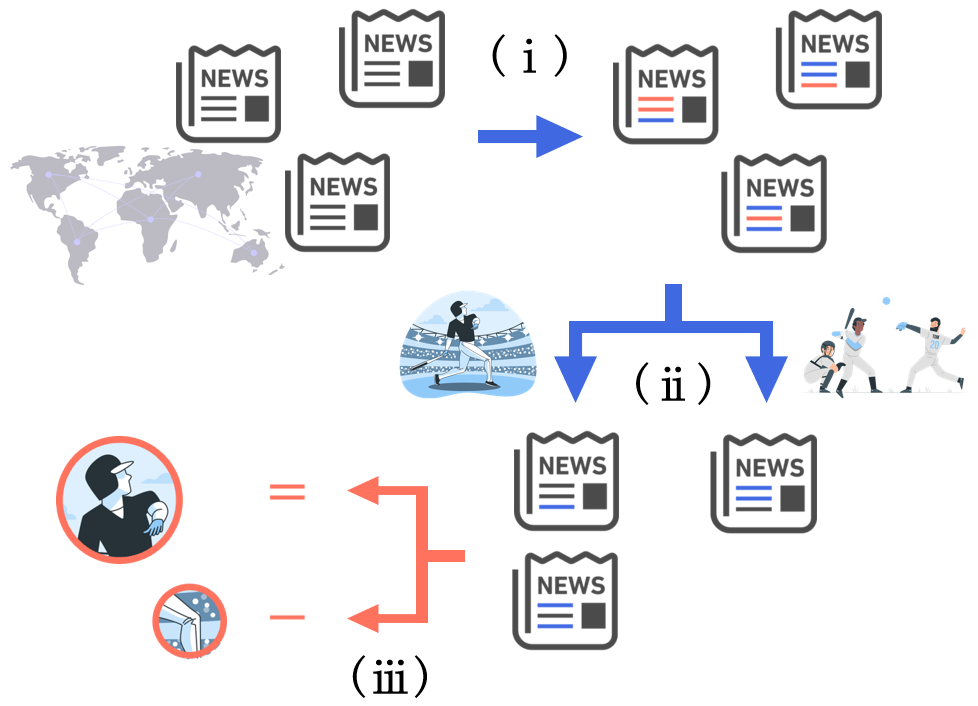
\includegraphics[keepaspectratio, width=60mm]{img/system_abstract.png}
	% 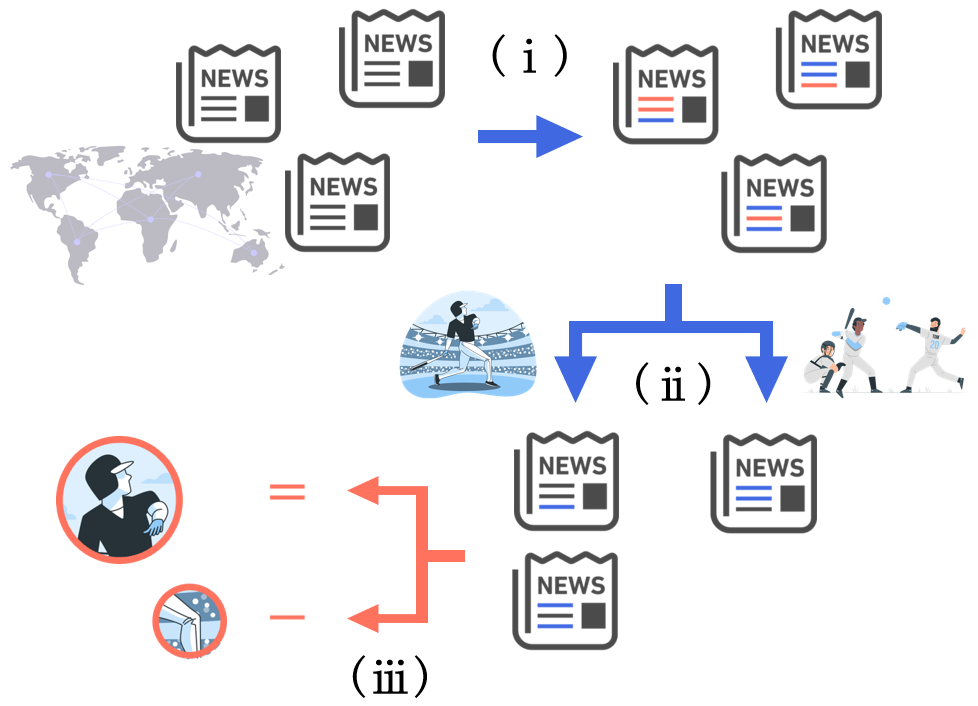
\includegraphics[keepaspectratio, width=60mm]{img/system_abstract.png}
	% 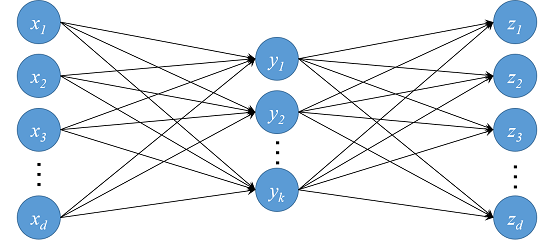
\includegraphics[keepaspectratio, width=60mm]{img/sample.png}
	\caption{
    提案手法のシステムの概要
    \\$\rm(\hspace{.18em}i\hspace{.18em})$
    記事の文章を出来事の文と主張の文に分類
    \\$\rm(\hspace{.08em}ii\hspace{.08em})$
    出来事の文章の類似度で記事をクラスタリング
    \\$\rm(i\hspace{-.08em}i\hspace{-.08em}i)$
    主張の文の類似度で主張の文をクラスタリング
  }
	\label{system_abstract}
\end{figure}


%%%%%%%%%%%%%%%%%%%%%%%%%%%%%%%%%%%%%%%%%%%
%% Section 関連研究
%%%%%%%%%%%%%%%%%%%%%%%%%%%%%%%%%%%%%%%%%%%
% \section{関連研究}
% 意味や話題が類似する文章の推薦手法として,LDA(Latent Dirichlet Allocation)~\cite{tian_labeled_2018}やSentence-BERT~\cite{reimers_sentence-bert_2019}が提案されている.
% LDAは記事に関連の深い単語群とそれぞれの単語の関連度を出力するが,単語群同士の関係性が得られないという点で,出来事の類似度が高い記事は得にくいと考えられる.
% 一方,Sentence-BERTは単語同士の関係性を加味した文意の数値ベクトルを出力するため,より高い出来事の類似度が得られると考えられる.
% しかし,記事の全文をSentence-BERTに入力した場合,出来事の類似度の算出に主張を述べる文も考慮することになり,より近い出来事に関する主張の違いを推薦できない.

% \begin{comment}
% SCDV, オントロジー, Transformer
% 潜在的意味,同義語
% トピック同士の関係が考慮されない
% 多言語に対応していない
% 主張に着目した研究は少ない
% 事象と主張が混在
% \end{comment}

% \begin{table}[h]
%   \caption{キャプション}
%   \label{table_a}
%   \centering
%   \begin{tabular}{lcr}
%     \hline
%     手法   & 正解率[\%]  &  計算時間[ms]  \\
%     \hline \hline
%     手法A  & 92.3  & 512 \\
%     手法B  & 87.4  & 32  \\
%     \hline
%   \end{tabular}
% \end{table}

%%%%%%%%%%%%%%%%%%%%%%%%%%%%%%%%%%%%%%%%%%%
%% Section 提案手法
%%%%%%%%%%%%%%%%%%%%%%%%%%%%%%%%%%%%%%%%%%%

\section{提案手法}

% \subsection{データセットの選定と前処理}
\subsection{RoBERTaによる出来事の文と主張の文の分類}
入力する記事には,Piyushらが収集したCOVID-19 News Articlesを選定した\cite{ghasiya_investigating_2021}.
COVID-19はフェイクニュースが多い話題であり,またインド,日本,韓国の7社の英記事が含まれるため,政治や文化の違いに由来する多くの異なる主張が分析できると考えた.
また,11カ月間という短い期間で収集されているため,より類似した出来事に関する記事が得られると考えた.
% 省略可能?
Yangらの研究と同様に話題がCOVID-19に限定されてしまっているが,限定された話題でも同じ出来事の異なる主張がグループ化される様子は観測できると考えた.
% @see weekly-report_20210930.md

% このとき
% また,記事の出来事をより類似させるため,同じ出稿日の記事を扱う.
% の各文章が,出来事と主張のどちらを述べているかを分類する.
本研究では,記事の文章が出来事を述べる文と主張を述べる文に二分できると仮定する.
% そして,出来事の文のみ,主張の文のみで2回に分けてクラスタリングすることで,より近い出来事に関する異なる主張の文の推薦を目指す.
出来事と主張の文の分類には,RoBERTaを応用した分類器を用いる.
RoBERTaは文意や文脈を加味した自然言語処理が可能な機械学習モデルで,GLUE,SQuAD,RACEといったベンチマークで2019年の最先端のスコアを有している\cite{liu_roberta_2019}.
ニュース記事を含む約160GBの文章データで事前に学習されたRoBERTa BASEモデルを利用し,これが分類タスクに特化するよう,主張か出来事かでラベル付けした文章で追加学習を行った.
% で,Dense層を加えたモデルのエンコード部分を用いることで分類タスクに応用できる.
% 入力部分にDense層を付加

追加学習には,Wikipediaの英文をClaimを述べるかEvidenceを述べるかでラベル付けしたRutyらのIBM Debater$^{\textregistered}$ - Claims and Evidenceを利用した\cite{rinott_show_2015}.
Claimは「トピックを直接サポートする一般的で簡潔な文」,Evidenceは「トピックの文脈の中でClaimを直接サポートする文章」と定義されており,本研究では主張とClaim,出来事とEvidenceを同じ定義で扱う.
表\ref{claim_evidence_example}にClaimとEvidenceの例を示す.

\begin{table}[h]
  \caption{IBM Debater$^{\textregistered}$ - Claims and Evidencでラベル付けされたClaimの文(C)とEvidenceの文(E)の例}
  \centering
  % \begin{tabular}{cp{6cm}}
  \begin{tabular}{llp{6cm}}
    \hline
    C & global carbon emissions are caused by de-
    \\
    & forestation
    % コンマがないのはデフォルト
    \\
    E & From 1990 to 2010 Nigeria nearly halved
    \\
    & their amount of Forest Cover, moving from
    \\
    & 17,234 to 9041 hectares.
    \\
    \hline
  \end{tabular}
  \label{claim_evidence_example}
\end{table}

システム全体の精度向上のため,2つのデータセットの前処理として
% 正規表現を用いた
小文字化やURLの除去などを行った.
また,文章中の文の区切り位置を同定するため,機械学習ライブラリStanzaによるテキスト解析を行った\cite{qi_stanza_2020}.
本システムにおいてStanzaはルールベースのspaCyよりも高速で,句点と句点以外のピリオドを精度良く区別できることを確認した.
% 省略可能
% StanzaはルールベースのspaCyに比べ,コンマに強い


%%%%%%%%%%%%%%%%%%%%%%%%%%%%%%%%%%%%%%%%%%%

\subsection{
Sentence-BERT,コサイン類似度,Ward法を用いた
出来事と主張の
階層的クラスタリング
% による出来事の文章と主張の文のグループ化
}

「出来事と分類した文を記事ごとに結合した文章」と「主張と分類した文」のそれぞれを,Sentence-BERTを用いてクラスタリングしやすい数値ベクトルに変換した.
Sentence-BERTは文章を文意を加味した数値ベクトルに変換できる機械学習モデルで,RoBERTaで65時間かかっていた文の類似度算出を約5秒に短縮し,STSタスク(Semantic Textual Similarity tasks)で2019年の最先端のスコアを有している\cite{reimers_sentence-bert_2019}.
事前に学習されたSentence-BERTのモデルには
% ,ライブラリにデフォルトで提供されている
paraphrase-MiniLM-L6-v2を使用した.
% 省略可能

文章の類似度の算出にはSentence-BERTの論文で用いられていたコサイン類似度を使用し,(Ward法について調べたこと,Ward法以外を試せたらそれについて書く)クラスタリングにはWard法を用いた.

/**

「根拠」のタイトル回収ができなていない

(出来事にすればよかった)

(出来事と主張の順にすればよかった)

(論文タイトルは変更できますか?)

**/

%%%%%%%%%%%%%%%%%%%%%%%%%%%%%%%%%%%%%%%%%%%
%% Section 評価実験
%%%%%%%%%%%%%%%%%%%%%%%%%%%%%%%%%%%%%%%%%%%
\section{評価実験}

/**

(バッチサイズ,エポック数,不均衡データ用のウェイト)

(IBMからcovidへの適用,IBMのラベルの傾向分析,独自の手付けラベル,不均衡データ用の正例の設定とMCC)


(クラスタリング結果の文の組の表)

(hとc?関連研究の相関分析?カイ二乗分布?)


分類精度

計算時間

良く見える結果

気になるエラー例

タイトル回収?

**/

%%%%%%%%%%%%%%%%%%%%%%%%%%%%%%%%%%%%%%%%%%%
%% Section 考察
%%%%%%%%%%%%%%%%%%%%%%%%%%%%%%%%%%%%%%%%%%%
\section{考察}

/**

手動ラベルの

バッチサイズの改善

T5の利用の検討

良く見える結果->妥当性

エラーの原因と対策

タイトル回収?

**/


%%%%%%%%%%%%%%%%%%%%%%%%%%%%%%%%%%%%%%%%%%%
%% Section まとめ
%%%%%%%%%%%%%%%%%%%%%%%%%%%%%%%%%%%%%%%%%%%
\section{まとめ}

/**

手法の目的を1文で説明

主にタイトル

何をしたか

結果何ができたか

課題

**/

%%%%%%%%%%%%%%%%%%%%%%%%%%%%%%%%%%%%%%%%%%%
%% Section 研究状況
%%%%%%%%%%%%%%%%%%%%%%%%%%%%%%%%%%%%%%%%%%%
% \section{研究状況}

% 分類精度の確認のため,前述の操作で出来事の文と主張の文の分類を行った.
% ただし,分類する日本の記事にはJapanese FakeNews Dataset中の偽物でないWikinewsを利用した~\cite{japanese_fakenews_dataset}.
% 学習で正解率が約0.993となったモデルで分類を行ったところ,表\ref{classify_result}の結果が得られた.


% \begin{table}[h]
%   \caption{Evidenceの文 ($E$) とClaimの文 ($C$) の分類結果}
%   \label{classify_result}
%   \centering
%   \begin{tabular}{cp{6cm}}
%     \hline
%     分類 & \multicolumn{1}{c}{翻訳前の入力文(一部抜粋)}  \\
%     \hline \hline
%     $E$  & 決勝のヒットを打った23日の試合も1球だけで終わった \\
%     $C$  & 日本シリーズ進出を決めてうれしい \\
%     \hline
%   \end{tabular}
% \end{table}

% 文$E$は,記者の解釈に依存しない,誰が観測しても不変な出来事を表している.
% また,文$C
% % , C_3, C_5
% $は,出来事に対する主張を表している.
% 一方で
% 文中に出来事を表す「敗れた」や「風が吹く」という言葉が含まれることより,出来事を誤分類したケースも見られた.

%%%%%%%%%%%%%%%%%%%%%%%%%%%%%%%%%%%%%%%%%%%
%% Section 今後の予定
%%%%%%%%%%%%%%%%%%%%%%%%%%%%%%%%%%%%%%%%%%%
% \section{今後の予定}

% 今後は,1文中の出来事と主張の要素を比率で考えるなどして,推薦精度を高めるように研究を進める予定である.

% 現在,主張を述べる文章を二重引用符を含む文章と仮定しているが,指示語や否定語の係り受けや引用符内の単語数によってはこの仮定は不適切である可能性がある.
% また,引用符の外の文章も主張を述べる文章である可能性があり,推薦の精度のために精査が必要である.
% 加えて,Transformerに代わるクラスタリング手法として,文意をベクトルで表現するLCDA(Sparse Composite Document Vectors)の利用も検討している.
% LCDAもまた主張の類似度を測るための手法ではないため,Trandsformerとのクラスタリングの精度の比較が必要である.

% を用いた → で
% (事象と主張以外の集合が存在する可能性)

\bibliographystyle{junsrt}
{\footnotesize \bibliography{ref.bib}}

\end{document}
